\documentclass[BCOR20mm,DIV14,10pt,headinclude,footexclude,bibtotoc,liststotoc]{article}

\makeatletter
\author{Jonas Otto} \let\theauthor\@author
\newcommand\matrikelnr{982249}
\newcommand\topicNrTitle{4: Parallelization}
\newcommand\theWordCount{2.000-3.000}


% Satzspiegel {{{
\renewcommand{\baselinestretch}{1.10}
\setlength{\parindent}{0pt}
\setlength{\parskip}{10pt}
\setlength{\baselineskip}{0pt}
\widowpenalty10000
\clubpenalty10000
% }}}

\usepackage[utf8]{inputenc}
\usepackage[USenglish]{babel}

\usepackage{graphicx}
\usepackage[automark]{scrlayer-scrpage}

\usepackage{todonotes}
\presetkeys{todonotes}{inline}{}

\usepackage{hyperref}

\usepackage{amsmath}

\usepackage{cleveref}

\usepackage{pgfplots}
\pgfplotsset{compat=1.17}

% Amdahl x ticks
\usepackage{xintexpr}

% Make clickable footnote
\newcommand{\hyperfootnote}[1][]{\def\ArgI{{#1}}\hyperfootnoteRelay}
 % relay to new command to make extra optional command possible
 \newcommand\hyperfootnoteRelay[2][]{\href{#1#2}{\ArgI}\footnote{\href{#1#2}{#2}}}
 % the first optional argument is now in \ArgI, the second is in #1

\begin{document}
\begin{titlepage}

	
\includegraphics[height=1.8cm]{images/logo_100_sw_bildmarke}
	\hfill
	
\includegraphics[height=1.8cm]{images/logo_100_sw_wortmarke}\\[1em]


	{\footnotesize
	\hspace*{8.25cm}{\bfseries Fakult{\"a}t f{\"u}r\\
		\hspace*{8.25cm}Ingenieurwissenschaften\\
		\hspace*{8.25cm}und Informatik}\\
	\hspace*{8.25cm}Institut f{\"u}r Organisation und\\
	\hspace*{8.25cm}Management von Informations-
	\hspace*{8.25cm}systemen\\[1em]
	}

	\vspace{10em}
	\begin{center}
		\begin{Large}
			\topicNrTitle \\
		\end{Large}
		\vspace{15em}
		\theauthor \\
		Matrikelnummer: \matrikelnr \\
		ENGG 72323 - Heterogeneous and Parallel Computing Infrastructures \\
		Wordcount: \theWordCount
	\end{center}

\end{titlepage}

\section{Introduction}
% \subsection{Topic Description}
% Parallelization. Since the processor speed is hardly increasing anymore, the
% only way to really improve performance of an application is to parallelize.
% Discuss the different ways in which an application can be parallelized and why
% and when which method is preferable. Do all parallel applications scale well?
% Which factors determine the performance / scalability of an application and
% how can you affect them when writing the application.

In recent history, processor performance indicators such as frequency seem to
have stagnated. At the same time however, the number of processing cores in a
single system has steadily increased (\cref{fig:processor_trend}). This prompts
software developers to adopt a mindset of thinking about parallelization while
shaping today's software landscape, to keep up with advances in processor and
computer design.

Not all applications are suited to all forms of parallelism, and the scalability
and expected performance gain is finite. In this essay, the different ways in
which an application can be parallelized, and the factors determining
scalability, will be presented and discussed.

\begin{figure}[h]
	\centering
	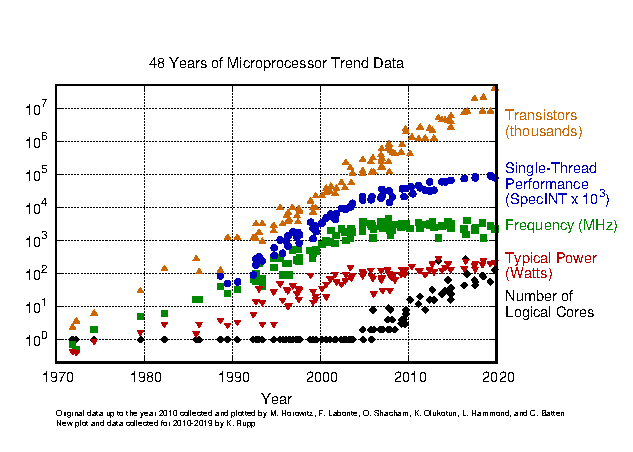
\includegraphics{images/48-years-processor-trend}
	\caption[48 Years of Microprocessor Trend Data]{
		\href{https://github.com/karlrupp/microprocessor-trend-data}
		{``48 Years of Microprocessor Trend Data''} by Karl Rupp, licensed under
		\href{https://creativecommons.org/licenses/by/4.0/}{CC BY 4.0}}
	\label{fig:processor_trend}
\end{figure}

\section{Analysis}

\subsection{Parallel Computing}
\label{sec:parallel_computing}
A classification of the many parallel computing architectures has been suggested
by Flynn. Flynn distinguishes computer architectures by the number of
instruction streams (Singe Instruction \emph{SI} or Multiple Instruction
\emph{MI}) and number of data streams (Single Data \emph{SD} or Multiple Data
\emph{MD}). Of the four resulting classifications, all but the \emph{MISD}
variant are commonly found, and of those the Single Instruction Multiple Data
\emph{SIMD} and Multiple Instruction Multiple Data \emph{MIMD} variants are of
interest to us here. Most commonly available processors for general purpose
computing follow a combination of those approaches: Multicore processors that
allow simultaneous execution of multiple programs on separate data (\emph{MIMD}
classification) are commonplace. Additionally, the individual processing cores
often offer \emph{vector extensions}, which as a form of \emph{SIMD} computing
offer fast mathematical operations on multiple values (vectors) at once.

Distributed systems such as entire HPC clusters may also be classified as
\emph{MIMD} computing architectures.

It is apparent that \emph{MIMD} architectures in particular are a very far
ranging classification, and lend themselves to more granular categorizing. A
useful distinction is between shared-memory and non-shared-memory systems. The
defining characteristic of a non-shared-memory system is the need for a
dedicated communication channel between multiple processing units. On a
shared-memory system, this communication can happen implicitly through memory
regions accessible to multiple processing units.

On the largest scale, such non-shared-memory, \emph{MIMD} systems such as high
performance clusters perform parallel computation by providing a large number of
nodes, that each run independently. A fast interconnect between the individual
nodes is usually present, but has to be used explicitly (using libraries such as
MPI for example).

Single processing nodes (or individual computers, for that matter) are
themselves \emph{MIMD} systems, but this time usually of the shared-memory
variant. All processors share common RAM, and the operating system provides
means of running parallel computation: Processes usually receive their own
protected memory segment for safety and security purposes, but multiple threads
inside one process can access the same memory without any operating system
intervention. The operating system provides scheduling for processes and threads
(and has no need to differentiate between a process and thread during
scheduling), which allows many programs and programs with more threads than
processors to run concurrently. The operating system periodically interrupts
execution and selects a different, waiting, thread for execution. Those context
switches can yield a substantial performance deficit when many threads are used,
and the ratio between program execution time and time spent switching threads is
bad.

\subsection{Task Parallelism}
\label{sec:task_parallel}
To benefit from the multiple ways of parallel computing described in
\cref{sec:parallel_computing}, an application has to be analyzed in which ways
it can be parallelized, and how it scales with an increasing degree of
parallelization, and with increasing problem size.

In order to explore and model the ways in which an application can be
parallelized, two models are usually considered: Task- and data parallelism.

In this first part, the concept of task parallelism is explored. If an
application consists of multiple individual tasks, those can be performed
according to its dependencies. \Cref{fig:task_graph} illustrates this in terms
of a data flow graph: In this example of an autonomous driving application, the
individual tasks all require some input data, which is provided by another task.
The tracking algorithm for example needs information about both the lane and
traffic signs in front of the vehicle. It is however apparent that the tasks of
creating a grayscale image and then detecting the lane and the task of creating
the RGB image and detecting traffic signs can be executed in parallel. They both
depend on the camera image, but execute independently. The serial part of the
application continues with the tracking step, which depends on the results of
all the previous detection steps. Planning can only be performed after the
tracking step.

\begin{figure}
	\centering
	\begin{tikzpicture}
    \node[draw, red] (camera) {Camera};
    \node[draw] (grayscale) [right=of camera] {Bayer to grayscale};
    \node[draw] (lane) [right=of grayscale] {Detect lane};
    \node[draw, red] (rgb) [below=of camera] {Bayer to RGB};
    \node[draw, red] (signs) [right=of rgb] {Detect signs};
    \node[draw, red] (tracking) [right=of signs] {Tracking};
    \node[draw, red] (planning) [right=of tracking] {Planning};
    \node[draw] (viz) [below=of rgb] {Visualization};
    \node[draw] (odom) [below=of tracking] {Odometry};

    \draw[->] (camera) -- (grayscale);
    \draw[->, red] (camera) -- (rgb);
    \draw[->] (grayscale) -- (lane);
    \draw[->] (lane) -- (tracking);
    \draw[->, red] (tracking) -- (planning);
    \draw[->, red] (rgb) -- (signs);
    \draw[->, red] (signs) -- (tracking);
    \draw[->] (rgb) -- (viz);
    \draw[->] (odom) -- (tracking);
\end{tikzpicture}

	\caption{Data flow graph of a fictional task-parallel autonomous-driving application}
	\label{fig:task_graph}
\end{figure}

The \emph{critical path} is the path of execution that determines the execution
time of the entire application. In \cref{fig:task_graph}, the critical path is
marked in red. No matter to which degree the application is parallelized, the
total execution time will never be less than the execution time of the critical
path, since it's inherently serial. In \cref{sec:amdahl}, this will be be called
the \emph{serial part} of the application. Another bottleneck arises from the
available resources: If, for example, the lane-detection and visualization tasks
both require exclusive access to the GPU, those tasks can not be executed in
parallel, even though the data dependencies would allow it, but sequentially or
in a switching manner (depending on the scheduling used). There exist frameworks
such as ``SMP Superscalar'' from the Barcelona Supercomputing Center \cite{hpci}
and the OpenCV Graph API that allow the programmer to directly specify the
different tasks and dependencies between them. The framework can then execute
tasks in parallel and start dependent tasks once their input is ready.


\subsection{Data Parallelism}
In data-parallel applications, only one single type of task is considered. This
task is however applied to a large amount of data, which can be split up to
parallelize the application. Common examples of data-parallel algorithms are
found in the field of image processing. When applying a filter in the form of
convolution with a filter kernel, each pixel in the resulting image could be
calculated simultaneously. It only depends on a part of the input image, and the
same operation is applied for each pixel.

It has to be ensured that no data dependencies exist between the individual
instances of the task, since tasks would have to wait for completion of the
previous one otherwise (see \cref{sec:task_parallel}).

One of the main difficulties in parallelizing a data-parallel application is the
segmentation of the data. A segmentation into the smallest possible parts, such
as individual pixels of an image, is usually far from optimal. Launching a
thread or process always incurs some fixed overhead, and running more threads
than processors available increases the overhead of context switching. Other
aspects of segmentation have to be kept in mind: Preserving data locality is
important to benefit from processor caches, and the particular form of
segmentation might help reduce communication, such as by only exchanging data at
the border of the segment between iterations. The optimal degree of
parallelization can often only be determined empirically.

\subsection{Scalability: Amdahl's Law}
\label{sec:amdahl}
Not every part of an application can be parallelized. In
\cref{sec:task_parallel}, it became apparent that tasks often depend on the
result of other tasks, which forces them to execute sequentially. In data
parallel applications, segmenting the dataset must be done before parallel
execution begins.

Named after the computer scientist Gene Amdahl, the maximum possible speedup of
an application that consists of a sequential part $s$ and a parallelizable part
$p=1-s$ can be determined using \emph{Amdahl's Law} \cite{amdahl1967}: Given $n$
cores or processors, an application which runs in time $t$ before
parallelization will have an execution time of
\begin{equation}
	t_\text{parallel} = s \cdot t + \frac{(1-s)\cdot t}{n}
\end{equation}
or slower.

Relating the original and parallelized execution time yields the total speedup
$S$:
\begin{eqnarray}
	S = \frac{t}{t_\text{parallel}} = \frac{n}{n \cdot s + (1-s)}
\end{eqnarray}

\begin{figure}
	\centering
	\begin{tikzpicture}
    \begin{axis}[
            width=\textwidth,
            height=0.5\textwidth,
            xmin=1, xmax=128,
            ymin=1, ymax=64,
            xtick={1,8,16,32,64,128},
            ytick={1,8,16,32,64},
            xlabel={Number of cores},
            ylabel={Speedup}
        ]
        \foreach [evaluate=\s as \redfrac using (\s*10)] \s in {0,2,...,10} {
                \edef\temp{\noexpand\addplot[thick, domain=1:128, samples=200, red!\redfrac!green]{x/(x * (\s/100) + (1-(\s/100)))};
                    \noexpand\addlegendentry{$s=\s\%$}}
                \temp
            }
    \end{axis}
\end{tikzpicture}

	\caption{Maximum application with increasing degree of parallelism, according to Amdahl's Law, for varying parts of non-parallelizable code}
	\label{fig:amdahl}
\end{figure}

This provides us with a theoretical upper bound for the speedup we can expect
when parallelizing an application.

Graphing this relationship of speedup by number of cores, for varying amounts of
serial part $s$, results in \cref{fig:amdahl}. It is apparent that even for
applications that are largely parallelizable, the benefit of adding additional
processing units diminishes quickly. \Cref{fig:amdahl_inverted} shows this
relationship for fixed $n$, and it is apparent that significant performance
gains require a sufficiently large parallelizable part.

\begin{figure}
	\centering
	\begin{tikzpicture}
    \begin{axis}[
            width=\textwidth,
            height=0.5\textwidth,
            xmin=75, xmax=100,
            xticklabel=\pgfmathprintnumber{\tick}\%,
            %ymin=1, ymax=55,
            %log basis x=2,
            xlabel={Parallel part},
            %xticklabel={\xinttheiexpr[0]2^\tick\relax},
            ylabel={Speedup},
            legend pos = north west
        ]
        \foreach [evaluate=\n as \redfrac using (\n*1.5)] \n in {64,32,16,4,1} {
                \edef\temp{\noexpand\addplot[thick, domain=75:100, samples=200, red!\redfrac!green]{\n/(\n * (1-x/100) + (x/100))};
                    \noexpand\addlegendentry{$n=\n$}}
                \temp
            }
    \end{axis}
\end{tikzpicture}
	\caption{Amdahl's law graphed for fixed $n$}
	\label{fig:amdahl_inverted}
\end{figure}


\subsection{Limitations of Amdahl's Law}
Amdahl's law provides an upper bound, but not one that a programmer can
reasonably expect to immediately reach. Even with trivially parallel problems,
the overhead induced by parallelizing is never zero. Communication, organization
and management of parallel execution threads takes time, and increases with the
number of threads. We expect to reach a point where the communication overhead
dominates the execution time compared to the actual application task. The
speedup decreases, and may even become negative, meaning the extra overhead
makes the parallel application run slower than the fully serial one. In
\cref{sec:parallel_computing}, it was already mentioned that an operating
system, which interrupts the running thread to run more threads than available
processors, can be devastating to performance. While the impact of the operating
system will not be discussed in detail here, this is important to consider when
designing parallel programs.

\section{Discussion}
In the following, the parallelization of applications shall be considered from
an implementation standpoint. How do the specific ways in which an application
exploits parallel computation differ? How does that impact the software design
and architecture? And in which layers of abstraction can the parallelization be
hidden?

\subsection{Parallelism at application level}
Direct, explicit parallelization of an application might be the most
straightforward way of running the program on a parallel architecture. This does
however mean that several challenges have to be addressed: Threads or processes
have to be started, the problem has to be partitioned, work has to be
distributed. Communication has to be established manually, and synchronization
between threads is necessary.

On this level, operating-system functions such as POSIX \texttt{pthreads} are
used for creating and managing threads. Synchronization primitives such as
semaphores or language specific implementations like the C++ \texttt{std::mutex}
are used to manage access to shared resources. Communication between threads can
be performed implicitly, by writing results into a shared memory segment or by
returning results directly.

A popular pattern for parallel applications is the \emph{fork-and-join} pattern:
The program repeatedly forks, spawning multiple threads that each work on a
portion of the current task, and then \emph{joins} those threads, waiting for
each to finish execution and thus providing a point of synchronization.

The \emph{master-worker} pattern describes a situation in which the work is
continuously packaged into tasks, which the \emph{master} then submits for
completion by a \emph{worker}. Both of these popular design patterns can be
combined, for example by submitting tasks to an existing thread pool instead of
actually \texttt{fork}ing the process or creating new threads, in order to avoid
some of the overhead induced by thread-creation.

An application programmer is however not required to use \texttt{pthreads} and
friends manually. Libraries such as Intel TBB and compiler extensions like
OpenACC \cite{openacc} and OpenMP \cite{openmp} exist and provide developers
with facilities like thread pools. OpenMP even offers automatic parallelization
of \texttt{for} loops for example, which implicitly divides the loop into tasks
submitted to the internal thread pool, and takes care of joining threads and
collecting results such that the program continues as if execution was
sequential.

\subsection{Parallelism below the application level}
In the interest of hiding implementation details from high-level programs,
parallelism can be hidden from the application programmer: If a software library
offers a sufficiently high level of abstraction, it can perform internal
operations in parallel while maintaining a serial programming model to the
developer. One example is the popular image processing library OpenCV: OpenCV
hides complex algorithms behind a relatively simple interface. Many of those
algorithms in the field of image processing lend themselves nicely to a
data-parallel approach and benefit greatly from parallelization. Therefore,
OpenCV maintains a thread pool to execute those operations, and even contains
GPU implementations using OpenCL and CUDA for some algorithms.

A similar approach is even taken by ubiquitous libraries such as the C++
\emph{Standard Template Library (STL)}: Since 2017, many of the functions in the
\texttt{<algorithm>} library take an additional \textit{execution policy}
argument that allows the programmer to specify that the algorithm shall be
parallelized, vectorized, both, or neither. The concrete implementation varies
by library vendor, but an internally maintained thread pool is used at least by
GCC`s \texttt{libstdc++} (using Intel TBB internally \cite{libstdc++}).

\subsection{Parallelism above the application level}
A different approach to parallelizing application code which is not written in
an inherently parallel way is to exploit the fact that the application may
already be divided into more or less independent modules, which can be executed
in parallel. This is often the case, when the application code is embedded into
some kind of framework. The Robot Operating System ROS for example is a
framework popular for application in the fields of robotics and automation. A
core concept of this framework is the notion of a node, which is a program that
receives and publishes data via publish/subscribe channels and performs a
specific task (such as receiving sensor data or controlling actuators). Those
nodes can be started in individual processes (or threads), since they only rely
on the publish/subscribe communication channels for synchronization.

While this can lead to an immediate performance increase compared to serial
execution, this does not provide scalability with more processors. The upper
bound of performance increase is reached as soon as every node has enough
processing resource to not have to share them with another node (disregarding
the potential of each single node to benefit from multiple processors).

A similar effect can be achieved using MPI, which also provides an inter-process
communication channel and starts multiple processes, although in this case the
individual processes usually perform the same task on a smaller subset of data,
which enables greater scalability with the number of processes. This could be
considered an example for data parallelism, while the ROS example is closer to
task parallelism.

\section{Conclusion}
Parallel processing architectures enable great advances in computational
performance despite stagnating clock speeds. To benefit from this development,
application programmers have to be aware of how execution time scales with an
ever increasing degree of parallelism, how to exploit the different ways a
computer architecture realizes parallel execution, and where the pitfalls lie
when programming a parallel system.

Amdahl's law illustrates how the effect of additional processing elements
diminishes the higher the inherently serial share of an application is. It
determines where the theoretical limits are in terms of expected speedup for a
given application with a varying degree of parallelism.

Task- and Data-Parallelism are two models that can be used to describe the
parallel nature of a problem, and help to transform that problem into a parallel
application. Finally, multiple approaches for specific implementations have been
discussed, from the viewpoint of a layered application utilizing frameworks and
libraries.

\newpage

\bibliographystyle{IEEEtran}
\bibliography{bibliography}

\cleardoublepage
\section*{Declaration of Originality}

I confirm that this assignment is my own work and that I have not sought or used
inadmissible help of third parties to produce this work and that I have clearly
referenced all sources used in the work. I have fully referenced and used
inverted commas for all text directly or indirectly quoted from a source.

This work has not yet been submitted to another examination institution –
neither in Germany nor outside Germany – neither in the same nor in a similar
way and has not yet been published.

\vspace{2cm}

Ulm, on the \dotfill

\hspace{10cm} {\footnotesize \theauthor}



\end{document}